\chapter{Mesh}
\section{Structure Analysis}
The device analyzed in this laboratory is a Double Quantum Dot structure fabricated using
Silicon MOS technology. The overall device has the dimensions as reported in the table \ref{dimensions}.

\begin{table}[ht]
\centering
\begin{tabular}{|c|c|}
\hline
Axis & Length (nm) \\
\hline
X & 353 \\
Y & 273 \\
Z & 126 \\
\hline
\end{tabular}
\caption{Device Dimensions}
\label{dimensions}
\end{table}

The device is divided into different regions determined by the code itself, in order to 
assign different properties both in terms of phyical caracteristics and in terms of meshing for 
the calculation of the simulation.\\
Regarding the mesh sizes, in the code are defined different measures that will be assigned to specific regions:
\begin{lstlisting}
        grid_spacing_01				= 1; //nm
	grid_spacing_02				= grid_spacing_01*2; 
	grid_spacing_03				= grid_spacing_02*2; 
	grid_spacing_04				= grid_spacing_03; 
	grid_spacing_05				= grid_spacing_03*2; 
\end{lstlisting}
Each of this parameter will indicates the local characteristic mesh size assigned to the points of the regions that will constitute the device. Of course, the higher the mesh size, the higher the elements size and so the lower of the mesh density, resulting in a lower accuracy when it comes to perform calcualtions.\\
Each point is defined as:
\begin{lstlisting}
    Point(id) = {x, y, z, lc};
\end{lstlisting}
where the last arguement is the one just mentioned.\\
By analyzing the code, it is possible to indentify the division of the structure, which is shown in table \ref{regions} starting from the bottom to the top,
with their respective mesh sizes.

\begin{table}[H]
\centering
\begin{tabular}{|c|c|}
\hline
Region name & Mesh size (nm) \\
\hline
region\_bulk\_bottom & 8 \\
region\_pre\_quantum\_A/B/C (bottom face)& 2 \\
region\_pre\_quantum\_A/B/C (top face)& 1 \\
region\_quantum\_A/B/C & 1 \\
region\_post\_quantum\_A/B/C & 2\\
region\_bulk\_top & 2 \\
region\_bottom\_oxide\_layer & 4 \\
region\_Y\_gate & 4 \\
region\_top\_oxide\_layer & 8 \\
region\_Barrier/Plunger/Reservoir\_X\_gate & 4 \\
\hline
\end{tabular}
\caption{Device regions and mesh sizes}
\label{regions}
\end{table}

As we can see, the regions with the highest mesh density are the ones that correponds to the volume of space where the quantum dots are located,
togheter with the regions right above and right below them. This is obvious, since here we need to calculate the poisson equation with the highest accuracy.


In order to have a better understanding of the overall structure,
we can observe the graphical representation in figure \ref{fullfigure} of the .geo file, in particular visualizing the 2D meshes, since with the 3D mesh is difficult to distinguish the different components.\\
\begin{figure}[H]
	\centering
	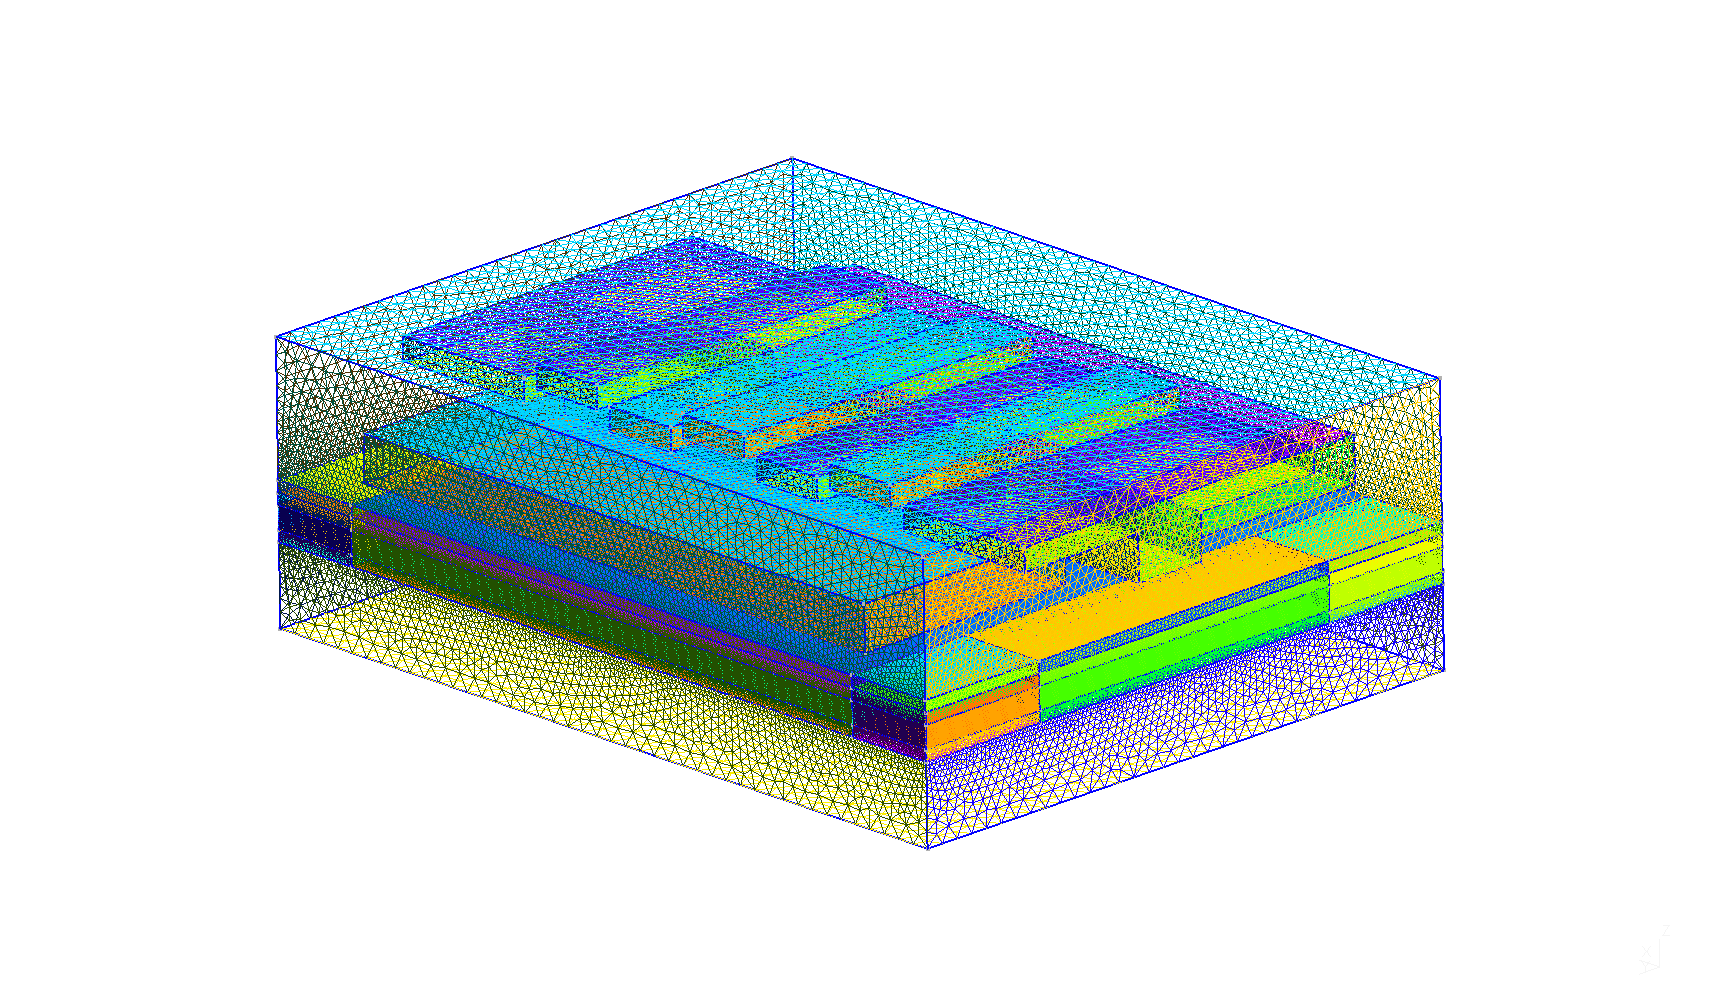
\includegraphics[width=1\textwidth]{Images/2Dfullfigure.png}
	\caption{2D mesh of the device}
	\label{fullfigure}
\end{figure}

Figure \ref{fullfigure} illustrates the two-dimensional mesh of the double quantum dot structure. As previously described, the mesh density varies across the different regions to optimize the computational accuracy and simulation time. Each functional region is clearly distinguishable due to a specific color.
It is worth to analyze the layout of the gates used in this type of double quantum dot structure: positioned directly above the active region, we find a pair of 'Y-gates' located at both ends of the y-axis (the short side). Their primary function is to provide lateral confinement, narrowing the silicon channel at the center of the device to create a quasi-one-dimensional path for electrons.
Above a thin dielectric layer, the 'X-gates' are visible. This layer includes three barrier gates—which define the tunnel junctions between the dots and the reservoirs, as well as the inter-dot barrier—and two plunger gates used to precisely tune the energy levels within each quantum dot. Additionally, two gates are positioned above the reservoir regions to regulate electron density and chemical potential.
A key feature of the X-gates is their characteristic T-shape. This geometry is designed to maximize the electrostatic coupling with the silicon channel. By partially wrapping around the sides of the channel, the T-shaped gates provide a more effective pinch-off compared to a simple planar gate. This ensures that the potential barriers are sharp and well-defined, which is critical for isolating individual electrons in the Coulomb blockade regime.